
\chapter{基于图像的树木轻量化3D建模方法}
\label{cha:techroute}

\section{技术路线}
\label{sec:techroute}
本文提出了一套完整的基于图像的树木轻量化3D建模的方法。该方法首先以树木图片
序列作为输入,用经过改进的方法对树木进行三维重建,使三维重建得到的模型精确
度和完整性都得以提高。然后再用基于空间方向迭代和步长探索的方法抽取树木的骨
架,最终再基于用户交互对骨架进行改善与轻量化。

该技术路线旨在实现一个对建模设备和条件要求不高,适用于一般应用的方法。在方便
和简单的基础上,尽可能多的加入自动化,并结合少量用户交互,以实现高效、精确的
树木轻量化3D建模。

该方法的主要步骤如下:

\subsection{基于改进的PyrLK光流法的图像特征匹配}
\label{subsec:match}
本文首先将著名的金字塔LK光流法(PyrLK)进行了改进和扩展,使本来以平面平移作为
运动假设的PyrLK光流法扩展为以平面仿射变换为运动假设,这样便能在两帧以空间角度
旋转而拍摄的图片中,捕捉到空间旋转变换的投影,提高了匹配的完整性和正确性。之后
本文再将得到的匹配点进行反向匹配,只有在一定容错区间内的匹配点对才会被接纳,并且
进行中值阈值,将邻域相似度小于中值以及反向匹配度小于中值的匹配对剔除,以提高匹配
算法的鲁棒性。

\subsection{三维重建}
\label{subsec:calibration}
特征匹配完成以后,本文使用了美国华盛顿大学西雅图分校Changchang Wu的可视化运动
恢复工具VisualSFM来完成基于多张图片的树木三维重建。VisualSFM实现了SiftGPU(GPU加速)
和多核的捆集调整(Multicore Bundle Adjustment), 使得相机参数的恢复更加
快速和精确。在这个步骤本文用经过改进的PyrLK光流法的匹配结果替换VisualSFM中的
SIFT特征点匹配文件,进一步地改进了相机参数恢复的准确度和可信度。

%\subsection{基于体素泛洪与空间反向投影的三维重建}
%\label{subsec:3drec}

\subsection{基于三维体素泛洪与线性拟合的三维树木骨架抽取}
\label{subsec:treesklextract}
在完成了三维重建之后,将会得到一个比较完整的树木空间点云模型。本文根据该点云的
空间分布,并结合树木自底向上的自然生长规律和分形的逻辑结构特征,在阈值范围内,
进行三维的体素泛洪,同时向多个子方向进行迭代,不断增加步长来扩大邻域范围。在确定
邻域以后将几个点数比例较大的方向作为分支方向,并用线性拟合的方法确定其精确的分支
方向。在确定分支方向后,再根据点到线的距离和投影分别估算出半径和长度。
同时在迭代过程中及时剔除已经形成枝干的点云,来加速泛洪算法的完成。最终获取到的骨架信息
是含有父子关系的节点信息,相比起3DSMAX等手工工具导出的面片模型,这种逻辑结构的
模型大大的减小了其尺寸,但是由于逻辑结构并没有多少丢失,所以极具真实感。并且这种
结构更便于后续的处理和进一步轻量化。

\subsection{基于用户交互的模型改善与轻量化}
\label{subsec:userinteraction}
由前面方法所得到的树木三维骨架虽然已经是含有父子信息的树木逻辑结构,但是由于前面
的步骤都是自动化生成,所得到的结果不可能100\%地保证符合具体应用的需求。并且前面的
骨架信息虽然比起用面片来表示树木模型已经大大的轻量化了,但是针对实际的应用,本文
还可以根据用户的交互来合并分支,从而进一步对模型进行轻量化,以适用于轻量化要求更
高的应用。

\subsection{建模质量评估}
\label{subsec:qualityevaluation}
对于一个通过建模获得的树木模型,如果没有一个客观的量化评价指标,就无法从客观的角度
反馈树木模型的还原度和各个步骤算法的可行性。本文提出了建模还原度的概念,以模型重建
的还原度来量化的表现建模的质量。该还原度分别计算输入图像序列的信息量、三维重建的还原
度和骨架抽取的还原度。并将它们有机地结合起来形成了最后总的建模还原度。

\section{技术路线图}
\label{sec:techrouteimg}
\begin{figure}[H]
	\centering
	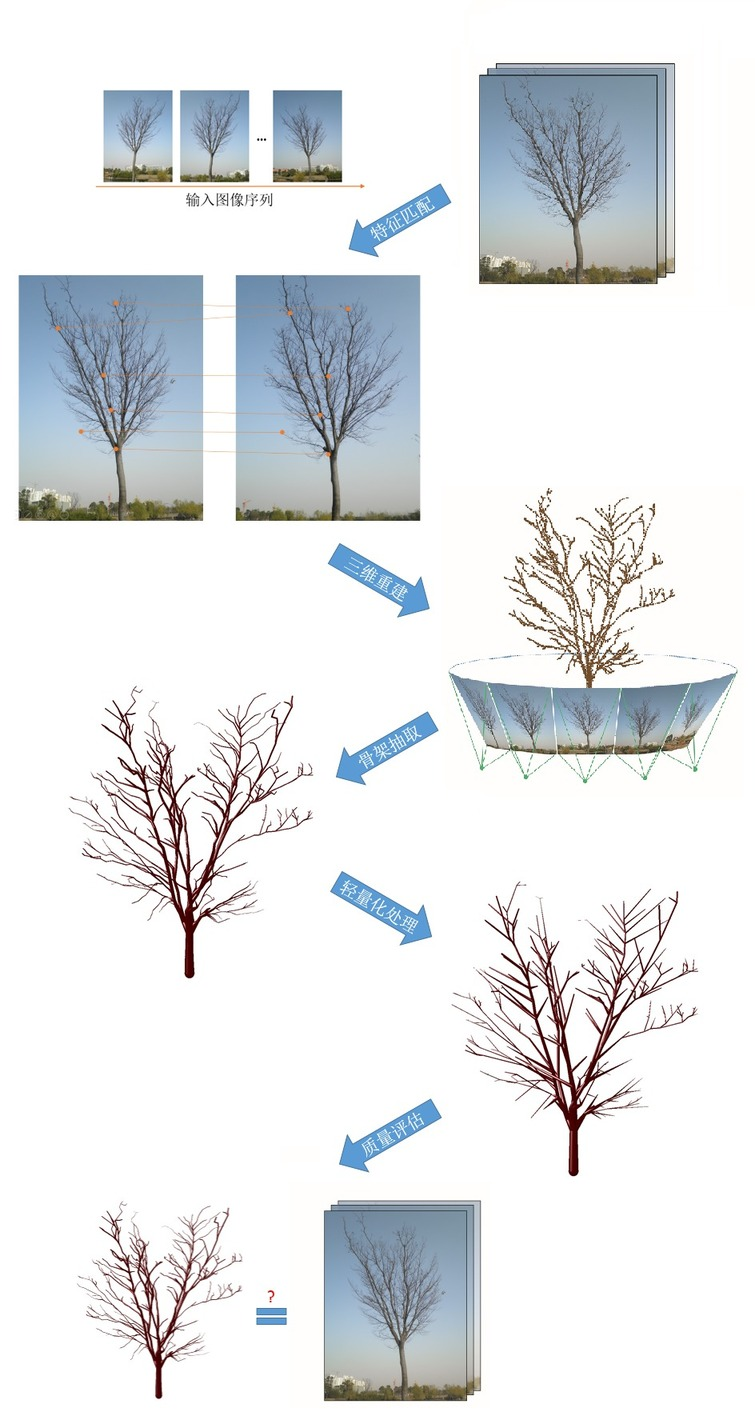
\includegraphics[height=20cm]{techroute.jpg}
	\caption{技术路线图}
	\label{fig:techroute}
\end{figure}
